\chapter{METHODOLOGY}
\section{Theoretical Background}
\subsection{Blockchain}
In general terms, a blockchain is an immutable transaction ledger, maintained within a distributed network of peer nodes. These nodes each maintain a copy of the ledger by applying transactions that have been validated by a consensus protocol, grouped into blocks that include a hash that bind each block to the preceding block.

\subsection{Permissioned vs Permissionless Blockchains}
Popular blockchain technologies like Bitcoin and Ethereum fall into a class of blockchain that we would classify as public permissionless blockchain technology. Basically, these are public networks where virtually anyone can participate, and every participant is anonymous.

In such a situation, the immutability of the blockchain's state up to a certain depth is the only possible foundation for trust. In order to mitigate this lack of trust, permissionless blockchains typically use a "mined" native cryptocurrency or transaction fees to provide economic incentive to offset the extraordinary costs of taking part in a byzantine fault-tolerant consensus based on "proof of work" (PoW).

Permissioned blockchains, on the other hand, operate a blockchain among a set of known, identified, and often vetted participants operating under a governance model that yields a certain degree of trust. A permissioned blockchain provides a way to secure the interactions among a group of entities that have a common goal but may not fully trust each other. By relying on the identities of the participants, a permissioned blockchain can use more traditional crash-fault-tolerant (CFT) or byzantine fault-tolerant (BFT) consensus protocols that do not require costly mining.

Furthermore, there is less chance of malicious code being purposefully introduced by a participant via a smart contract in such a permissioned environment. First, the participants are known to one another, and all actions, whether submitting application transactions, modifying the configuration of the network, or deploying a smart contract, are recorded on the blockchain following an endorsement policy that was established for the network and relevant transaction type. Rather than being completely anonymous, the guilty party can be easily identified, and the incident can be handled in accordance with the terms of the governance model.

\subsection{Hyperledger Fabric}
Hyperledger Fabric is an open source enterprise-grade permissioned distributed ledger technology (DLT) platform, designed for use in enterprise contexts, that delivers some key differentiating capabilities over other popular distributed ledger or blockchain platforms.It has a highly modular and configurable architecture, enabling innovation, versatility and optimization for a broad range of industry use cases.

Fabric supports smart contracts authored in general-purpose programming languages such as Java, Go and Node.js, rather than constrained domain-specific languages (DSL).

The Fabric platform is also permissioned, meaning that, unlike with a public permissionless network, the participants are known to each other, rather than anonymous and therefore fully untrusted. This means that while the participants may not fully trust one another (they may, for example, be competitors in the same industry), a network can be operated under a governance model that is built off of what trust does exist between participants, such as a legal agreement or framework for handling disputes.

One of the most important of the platform’s differentiators is its support for pluggable consensus protocols that enable the platform to be more effectively customized to fit particular use cases and trust models. Fabric can leverage consensus protocols that do not require a native cryptocurrency to incent costly mining or to fuel smart contract execution. Avoidance of a cryptocurrency reduces some significant risk/attack vectors, and absence of cryptographic mining operations means that the platform can be deployed with roughly the same operational cost as any other distributed system.

The combination of these differentiating design features makes Fabric a better choice both in terms of transaction processing and transaction confirmation latency, and it enables privacy and confidentiality of transactions and the smart contracts that implement them\cite{manevich2019endorsement}.
\subsection{Assets}
Assets can range from the tangible (real estate and hardware) to the intangible (contracts and intellectual property). Hyperledger Fabric provides the ability to modify assets using chaincode transactions. Assets are represented in Hyperledger Fabric as a collection of key-value pairs, with state changes recorded as transactions on a Channel ledger. Assets can be represented in binary and/or JSON form. Digital identity documents, which are stored in JSON format, are the asset in context of this project.
\subsection{Ledger}
The ledger is the sequenced, tamper-resistant record of all state transitions in the fabric. State transitions are a result of chaincode invocations (‘transactions’) submitted by participating parties. 
Each transaction results in a set of asset key-value pairs that are committed to the ledger as create, update, or delete operation is executed. 
In Hyperledger Fabric, a ledger consists of two distinct, though related, parts – a world state and a blockchain. 
Firstly, there’s a world state – a database that holds current values of a set of ledger states. The world state makes it easy for a program to directly access the current value of a state rather than having to calculate it by traversing the entire transaction log. Ledger states are, by default, expressed as key-value pairs. The world state can change frequently, as states can be created, updated and deleted.
Secondly, there’s a blockchain – a transaction log that records all the changes that have resulted in the current world state. Transactions are collected inside blocks that are appended to the blockchain – enabling you to understand the history of changes that have resulted in the current world state. The blockchain data structure is very different to the world state because once written, it cannot be modified; it is immutable.\newline
It’s helpful to think of it as one logical ledger existing for each channel in the network. In reality, each peer in a channel maintains its own copy of the ledger – which is kept consistent with every other peer’s copy through a process called consensus. The term Distributed Ledger Technology (DLT) is often associated with this kind of ledger – one that is logically singular, but has many identical copies distributed across a set of network nodes (peers and the ordering service).
\subsection{Chaincode (Smart Contract)}
Chaincode is software defining an asset or assets, and the transaction instructions for modifying the asset(s). In other words, it’s the business logic. Chaincode enforces the rules for reading or altering key-value pairs or other state database information. Chaincode functions execute against the ledger’s current state database and are initiated through a transaction proposal. Chaincode execution results in a set of key-value writes (write set) that can be submitted to the network and applied to the ledger on all peers.
\subsection{Consensus}
Consensus is defined as the full-circle verification of the correctness of a set of transactions comprising a block. Consensus is achieved ultimately when the order and results of a block’s transactions have met the explicit policy criteria checks. These checks and balances take place during the lifecycle of a transaction, and include the usage of endorsement policies to dictate which specific members must endorse a certain transaction class, as well as system chaincodes to ensure that these policies are enforced and upheld. It is a broader term overarching the entire transactional flow, which serves to generate an agreement on the order and to confirm the correctness of the set of transactions constituting a block. The consensus mechanism depends on the ordering service used.
\subsection{Raft}
Raft is the go-to ordering service choice for Hyperledger Fabric. Fabric implementation of the Raft protocol uses a “leader and follower” model, in which a leader is dynamically elected among the ordering nodes in a channel and that leader replicates messages to the follower nodes. Because the system can sustain the loss of nodes, including leader nodes, as long as there is a majority of ordering nodes (what’s known as a “quorum”) remaining, Raft is said to be “crash fault tolerant” (CFT). In other words, if there are three nodes in a channel, it can withstand the loss of one node (leaving two remaining). If you have five nodes in a channel, you can lose two nodes (leaving three remaining nodes). This feature of a Raft ordering service is a factor in the establishment of a high availability strategy for the ordering service\cite{honar2021hyperledger}.
\subsection{Endorsement policy}
Endorsement policy defines the peer nodes on a channel that must execute transactions attached to a specific chaincode application, and the required combination of responses (endorsements). A policy could require that a transaction be endorsed by a minimum number of endorsing peers, a minimum percentage of endorsing peers, or by all endorsing peers that are assigned to a specific chaincode application. Policies can be curated based on the application and the desired level of resilience against misbehavior (deliberate or not) by the endorsing peers. A transaction that is submitted must satisfy the endorsement policy before being marked as valid by committing peers\cite{androulaki2019endorsement}.
\subsection{Security \& Membership Services}
Hyperledger Fabric underpins a transactional network where all participants have known identities. Public Key Infrastructure is used to generate cryptographic certificates which are tied to organizations, network components, and end users or client applications. As a result, data access control can be manipulated and governed on the broader network and on channel levels. This “permissioned” notion of Hyperledger Fabric, coupled with the existence and capabilities of channels, helps address scenarios where privacy and confidentiality are paramount concerns.
\subsection{Membership Service Provider}
Certificate Authorities issue identities by generating a public and private key which forms a key-pair that can be used to prove identity. This identity needs a way to be recognized by the network, which is where the MSP comes in. For example, a peer uses its private key to digitally sign, or endorse, a transaction. The MSP is used to check that the peer is allowed to endorse the transaction. The public key from the peer’s certificate is then used to verify that the signature attached to the transaction is valid. Thus, the MSP is the mechanism that allows that identity to be trusted and recognized by the rest of the network.


\section{System Architecture}
\subsection{Test network} 
\vspace{10pt}
\begin{figure}[H]
\centerline{\includesvg[inkscapelatex=false,width=1\columnwidth]{images/methodology/TestArchitecture.svg}}
\caption{Architecture of the Test Network}
\label{fig: example}
\end{figure}
Hyperledger Fabric is used in this project to set up a test network of private blockchain. This test network is simulated in containers using Docker Compose. This test network is configured to contain two organizations, ’Parichaya’ and ’Nepal Government’. 
Parichaya represents the organization that interacts with the blockchain to provide digital identity services through the Parichaya App. Nepal Government represents the organization that interacts with the blockchain to maintain the digital record of government issued identity documents.

\textbf{Certificate Authority} \newline
Each organization has their own certificate authorities, CA1 for Parichaya and CA2 for Nepal Government. These CAs are responsible for dispensing certificates that can be used to identify components as belonging to an organization and also to sign transactions to indicate that an organization endorses the transaction result – a precondition of it being accepted onto the ledger. 

\textbf{Peers and Channels} \newline
Hyperledger has a concept of creating a channel where multiple organizations can collaborate to maintain a shared copy of ledgers to keep record of digital assets. In our testnet, we have two organizations, ’Parichaya’ and ’Nepal Government’, who agree on a channel configuration to jointly collaborate on a channel named “digital\_identity”.
For this both organizations host one peer each and both these peers are connected to this “digital\_identity” channel. These peers are a fundamental element of the network because they host ledgers and chaincode (which contain smart contracts) and are therefore one of the physical points at which organizations connect to the channel. 

\textbf{Chaincode} \newline
In Hyperledger Fabric, the business logic that defines how peer organizations interact with the ledger (for example, a transaction that adds a new category in a driving license record), is contained in a smart contract. The structure that contains the smart contract, called chaincode, is installed on the relevant peers, approved by the relevant peer organizations, and committed on the channel. In this way, we can consider a chaincode to be physically hosted on a peer but logically hosted on a channel. In our testnet, we have three chaincodes, nationalIdentity\_chaincode'', “citizenship\_chaincode” and “drivingLicense\_chaincode”, installed on every peer. “nationalIdentity\_chaincode'' contains the smart contracts for storing and updating the details of the National Identity Card. “citizenship\_chaincode" contains the smart contracts related to Citizenship Certificates. And “drivingLicense\_chaincode" contains the smart contracts related to Driving License. An endorsement policy has also been set for these chaincode, stating that both “Parichaya” and “Nepal Government” must endorse any transaction.

\textbf{State Database} \newline
Various data update transactions are appended to the distributed ledger on a regular basis. In such a situation, querying the entire ledger to get the latest state of the data is very computationally expensive. So instead a global state is maintained to keep the record of the latest state of the data in the ledger and such state is stored in the state database.\newline
World state data is stored in a state database for efficient reads and queries from chaincode. Both organizations maintain an instance of a database for this purpose.
CouchDB is used as the state database in our test network.

\textbf{Ordering Service} \newline
The ordering service gathers endorsed transactions from applications and orders them into transaction blocks, which are subsequently distributed to every peer node in the channel. At each of these committing peers, transactions are recorded and the local copy of the ledger updated appropriately. A single node Raft ordering service is configured with a maximum of 10 transactions per block and maximum elapsed duration for a block is set to 2 seconds.
% \end{itemize}
\subsection{The Gateway}
\vspace{15 pt}
\begin{figure}[H]
\centerline{\includesvg[inkscapelatex=false, angle=90, width=1.3\columnwidth]{images/methodology/GatewayArchitecture.svg}}
\caption{Architecture of the Gateway Application}
\label{fig: GatewayArchitecture.svg}
\end{figure}
\newpage
Just like peers and orderers, gateway application has an identity that associates it with an organization. In our testnet, one gateway application is associated with “Parichaya” Organization and another gateway application is associated with “Nepal Government” Organization. Both of these applications are then connected to the digital\_identity channel. 

Because Fabric is a permissioned network, blockchain participants need a way to prove their identity to the rest of the network in order to transact on the network. Hence, only after the gateway application has registered and enrolled with its associated organization’s Certificate Authority (CA) and received back necessary cryptographic material, can they use it to authenticate into the blockchain network. 

Hyperledger Fabric provides Node SDK with various APIs available to interact with the chaincode. Our gateway application leverages these APIs to create gRPC connection with the blockchain and perform various read/write operations.

To create a simple interaction mechanism with the blockchain we have wrapped these SDK APIs with our own set of APIs so that these read-write operations can be performed with a simple set of REST API calls. These REST APIs from the node server can be called by other applications to interact with the private blockchain.
\subsection{Karmachari App}
\vspace{15 pt}
\begin{figure}[H]
\centerline{\includesvg[inkscapelatex=false,width=1\columnwidth]{images/methodology/KarmachariArchitecture.svg}}
\caption{Architecture of the Karmachari App}
\label{fig: KarmachariArchitecture.svg}
\end{figure}
The Karmachari web application is connected to the blockchain through the Gateway Application for “Nepal Government”. This application will allow government officials to record and update the user identity details of National Identity Card, Citizenship Certificate and Driving License in the private blockchain.
% \newpage

\subsection{Parichaya App}
\vspace{15 pt}
\begin{figure}[H]
\centerline{\includesvg[inkscapelatex=false,width=1\columnwidth]{images/methodology/ParichayaArchitecture.svg}}
\caption{Architecture of the Parichaya App}
\label{fig: ParichayaArchitecture.svg}
\end{figure}
Parichaya mobile app allows a user to view all their identity documents stored by the government in the blockchain and also to share their documents or details with others through qr code. All of the data and services required by the mobile app are facilitated by the Parichaya backend server. This backend server can interact with the private blockchain through the Gateway Application for Parichaya.
\newpage
\begin{figure}[H]
\centerline{\includesvg[inkscapelatex=false,angle=90, width=1.6\columnwidth]{images/methodology/SystemArchitecture.svg}}
\caption{Architectural overview of the entire system}
\label{fig: SystemArchitecture.svg}
\end{figure}
\newpage
\section{Design and Implementation Details}
\vspace{15pt}
\subsection{Transaction Flow in blockchain}
\vspace{22pt}
\begin{figure} [H]
    \centering
    % 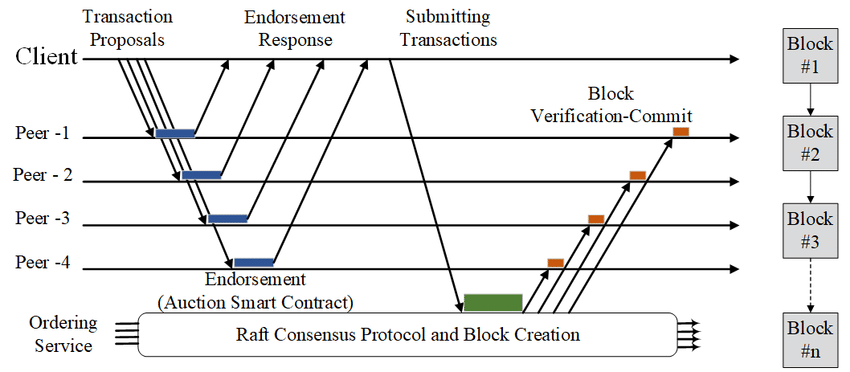
\includegraphics[width = 1\columnwidth]{images/methodology/TransactionFlow.jpg}
  \centerline{\includesvg[inkscapelatex=false, width=1\columnwidth]{images/methodology/TransactionFlow.svg}}
    \caption[Transaction flow in Hyperledger fabric]{Transaction flow in Hyperledger fabric}
    \label{fig:TransactionFlow.jpg}
\end{figure}

\textbf{Transaction initiation} \newline
Any transaction initiated by the gateway application targets the peers, who are the representative of the respective gateway applications. Peer of “Parichaya” is the target peer for the gateway application of “Parichaya” and Peer of “Nepal Government” is the target peer for the gateway application of “Nepal Government”.

For this, a transaction proposal is constructed first. The proposal is a request to invoke a chaincode function with certain input parameters, with the intent of reading and/or updating the ledger. The gateway application leveraging the Node SDK provided by hyperledger fabric utilizes one of the available API’s to generate the transaction proposal.

The SDK serves as a shim to package the transaction proposal into the properly architected format (protocol buffer over gRPC) and takes the application’s cryptographic credentials to produce a unique signature for this transaction proposal. The SDK submits the transaction proposal to a target peer, which will manage the transaction submission on behalf of the gateway application. The target peer first forwards the transaction proposal to other peers for execution, as required by the endorsement policy.\\ \newline

\textbf{Verification of Signature and Execution of transaction by Endorsing Peers} \newline
Both the endorsing peers, “Parichaya” and “Nepal Government” verify that the transaction proposal is well formed,  it has not been submitted already in the past (replay-attack protection),  the signature is valid (using the MSP), and  that the submitter (Gateway Application) is properly authorized to perform the proposed operation on that channel (digital\_identity channel). The endorsing peers take the transaction proposal inputs as arguments to the invoked chaincode’s function. The chaincode is then executed against the current state database to produce transaction results including a response value, read set, and write set (i.e. key/value pairs representing an identity document to create or update). No updates are made to the ledger at this point. The set of these values, along with the endorsing peer’s signature is passed back as a “proposal response” to the target peer.

\textbf{Inspection of proposal responses} \newline
The target peer verifies the proposal responses are the same prior to proceeding with the transaction submission. The architecture is such that even if a transaction is submitted without this check, the endorsement policy will still be checked and enforced when each peer validates transactions prior to committing them in the ledger.

\textbf{Assembly of endorsements into a transaction by target peer} \newline
The target peer “broadcasts” the transaction proposal and response within a “transaction message” to the ordering service. The transaction contains the Channel ID, the read/write sets, and a signature from each endorsing peer. The ordering service does not need to inspect the entire content of a transaction in order to perform its operation, it simply receives transactions, orders them, and creates blocks of transactions per channel.

\textbf{Transaction validation and commitment} \newline
The blocks of transactions are “delivered” to all peers on the channel. The transactions within the block are validated to ensure endorsement policy is fulfilled and to ensure that there have been no changes to ledger state for read set variables since the read set was generated by the transaction execution. Transactions in the block are tagged as being valid or invalid.\\\\

\textbf{Ledger update} \newline
Each peer appends the block to the channel’s chain, and for each valid transaction the write sets are committed to the current state database. An event is emitted by each peer to notify the gateway application that the transaction (invocation) has been immutably appended to the chain, as well as notification of whether the transaction was validated or invalidated.




\subsection{Implementation Details of Karmachari Web App}
\vspace{15pt}
    \begin{figure}[H]
\centerline{\includesvg[inkscapelatex=false,width=1\columnwidth]{images/methodology/KarmachariUsecase.svg}}
\caption{Use case Diagram of Karmachari Web App}

\label{fig: KarmachariUsecase.svg}
\end{figure}


Karmachari Web App provides an interface for the government officials to record and update the identity details of the users in the private blockchain. Initially, the users need to log in with their username and password. The credentials provided are then verified by the backend server before the user gets access to the main dashboard. Once the user is logged in, they can register the National Identity, Citizenship and Driving License of the users. They can also search for the required documents using the National Identity Number linked with it. Moreover, the users can update the searched document if necessary. \\\\
    

\textbf{Authentication}\newline
    Authentication process of the government officials on the web application is based on JWT authentication. For the login process in the web app, the user is required to input their username and password. The credentials are then forwarded to the node backend server for authentication through an API request. The backend server verifies the credentials and generates a JWT which is then returned back to the user as a response. On receiving the token, the user is logged in to the web application. The web app then attaches this authentication token with all other subsequent requests made by the web app to the backend.

\textbf{Registration of Documents} \newline
The government officials, after authentication, can fill the documents of the users on the Karmachari web app for registration. Initially, the officials have to fill the forms of national identity documents among others, as it acts as a base for all other documents. The form is validated during the filling process itself. The Karmachari web app then sends the document details to the Fabric gateway, which invokes a function on the smart contract to register the national identity document. However, for other documents, the government officials have to first enter the associated National Identity Number, The karmachari web app sends this number to the Fabric gateway which invokes a function on smart contract to check where the received National Identity Number exists on the blockchain or not. If it exists, the government officials are able to fill the form. Again, the form is validated during the process. Finally, the Karmachari web app sends the document details to the Fabric gateway, which invokes a function on the smart contract to register the required document.
    \begin{figure}[H]
\centerline{\includesvg[inkscapelatex=false,width=0.45\columnwidth]{images/methodology/RegisterNID.svg}}
\caption{Register NID}

\label{fig: example}
\end{figure}
   \begin{figure}[H]
\centerline{\includesvg[inkscapelatex=false,width=0.45\columnwidth]{images/methodology/RegisterLicense.svg}}
\caption{Register License}

\label{fig: RegisterLicense.svg}
\end{figure}

   \begin{figure}[H]
\centerline{\includesvg[inkscapelatex=false,width=0.45\columnwidth]{images/methodology/RegisterCitizenship.svg}}
\caption{Register Citizenship}

\label{fig: example}
\end{figure}

   
\textbf{Searching and Updating Documents}\newline
To search for any documents in the web app, the user needs to provide the National Identity Number of the user and select the document type the user is searching for. The web app then sends an API request to the backend server to check if the document exists, which in turn invokes a smart contract function in the blockchain through gRPC to check if the document exists. A response is then sent back to the web app. If the document exists, the details of the document are shown to the user. Else, an error is shown. The user can also update the details of the shown document if necessary. If the details are updated, the updated details are sent to the backend server which then overwrites the details of the document stored in the blockchain by invoking a smart contract function.\newline
Government official’s authentication on the web application is based on JWT authentication. The user inputs their username and password which is forwarded to the node backend server. The server verifies the credentials and generates a JSON Web Token. The server provides the token to the user as a response and the user is logged in to the web application. The user can then fill the forms (National Identity) of users into the blockchain storage through the server.
\begin{figure}[H]
\centerline{\includesvg[inkscapelatex=false,width=0.45\columnwidth]{images/methodology/SearchAndUpdate.svg}}
\caption{Search And Update Documents}

\label{fig: SearchAndUpdate.svg}
\end{figure}

\subsection{Implementation Details of Parichaya app}
\vspace{15pt}
\begin{figure}[H]
\centerline{\includesvg[inkscapelatex=false,width=1\columnwidth]{images/methodology/MobileUsecase.svg}}
\caption{Use Case Diagram of Parichaya App}
\label{fig: MobileUsecase.svg}
\end{figure}
Parichaya Mobile App provides an interface for users to view and share their identity document details. The user requires to be authenticated in the mobile app through their National Identity Number and mobile number.This process includes the user receiving an OTP in their registered mobile number. The user is authenticated if the input OTP is verified by the backend server. After authentication, users can view their government issued documents, online or offline. Moreover, users can share their identity details to other users or third party applications through QR code. Consequently, the users can also view other user’s identity details by scanning the QR code using the application’s scanner.\\ \\ 

\textbf{Authentication} \newline
The authentication process begins when the user provides their National Identity Number to the mobile app. The number is then forwarded to the Parichaya backend server and subsequently to the Fabric gateway application. The Fabric gateway invokes a function in the smart contract providing the number it received from the user. The function checks if the number exists in the blockchain and returns a response to the Fabric gateway. The response traverses all the way back to the mobile application, which shows an error or shows the next step of the authentication process depending on the response. The user then provides their Mobile Number, associated with their National Identity Card. The mobile number and the national identity number are forwarded to the Parichaya backend server, which requests for the National Identity Details of the given NIN to the Fabric gateway. The gateway invokes another function which provides the National Identity Details of the given NIN. This response traverses back to the Parichaya backend, where the mobile number it received is compared with the one in the National Identity Details. This is to check that the mobile number being used is indeed the mobile number that is linked with the National Identity Card. If it is verified, then an OTP is generated and sent to the given mobile number. The user is required to input the OTP, which is forwarded to the Parichaya backend. If the OTP is verified, an auth token is generated and sent as the response to the mobile app. The received token is then stored in the mobile database as all the future interactions with the Parichaya backend requires it for authentication. Finally, for app lock purposes, the user is required to set up a four digit pin code, which is stored in the mobile database as well. After the completion of each of these steps, the user is finally logged in to the mobile app.
    
\textbf{Fetching Documents}\newline
In the first login, a request for the government issued documents is sent to the Parichaya backend, including the NIN and the auth token. If the token has not expired, the same request is sent to the Fabric gateway. This invokes a function which returns a response containing all the available documents associated with the NIN. After the Parichaya backend obtains the response, it creates card images of each of the documents, front and back, for a better visual representation. The mobile app finally receives the documents along with the document images. The received documents and images are stored in the mobile database for offline viewing. Current date and time of the fetch request is also stored to sync the data in the mobile database with the data in the blockchain.\newline
For other subsequent logins, the user just has to input the pin code that was previously set. Users can also opt to enable biometric login options, which can be enabled from the settings of the mobile app. After verification, if there is no internet connection, the documents stored in the mobile database are shown, else if there is internet connection, then a syncing process is initiated. The syncing process starts by requesting for the last updated date and time of documents to the Parichaya backend, which includes sending the NIN and the auth token. If the token is valid, the mobile app acquires the date and time of the last update, which is compared to the one stored in the mobile database. If the mobile stored date and time is more recent than the fetched date and time, the currently stored documents in the mobile app are shown, else the process of document fetch is initiated.
  \begin{figure}[H]
\centerline{\includesvg[inkscapelatex=false,height=0.6\paperheight]{images/methodology/MobileActivity.svg}}
\caption{Activity Diagram Of Login Process in Parichaya App}

\label{fig: MobileActivity.svg}
\end{figure}
  \begin{figure}[H]
\centerline{\includesvg[inkscapelatex=false,width=1\columnwidth]{images/methodology/MobileAuthenticationSequence.svg}}
\caption{Authentication and Data Fetching Process in Parichaya App}

\label{fig: example}
\end{figure}


\textbf{Sharing Identity Details to Third Party Application} \newline
To send details to the third party web client, the user has to click on the apply with Parichaya button. This initiates a websocket connection between the web client and the Parichaya backend server. However, the web client has to be registered into the backend with their name, domain, logo and requesting identity fields. In other words, the backend has to recognize the third party client application before it can make a websocket connection. Otherwise, the request to establish the websocket connection is rejected by the Parichaya backend. After the initialization of websocket connection, the Parichaya backend responds with the request id. The web client generates a QR code using this request id. The user requires the Parichaya mobile app to scan the QR code, and once the QR code is scanned, the Parichaya app requests the Parichaya backend with the obtained request id for the details of the document requester and the requested fields. This is for the full transparency of the users data being shared. The user then chooses to either approve or deny this request after viewing the details of the document requester and the requested fields. If the user chooses to deny the request, the websocket connection closes by sending a denied message to the web client. If the user chooses to approve the request, the Parichaya backend requests for all the required user details to the Fabric gateway which invokes a function in the smart contract that responds with the required details. Finally, the Parichaya backend sends the user’s details to the web client. The websocket connection is then closed with an approved request message shown on the Parichaya app. \\


\begin{figure}[H]
\centerline{\includesvg[inkscapelatex=false,width=1\columnwidth]{images/methodology/ThirdpartyQRSequence.svg}}
\caption{Sharing Identity Details to Third Party Application}

\label{fig: ThirdpartyQRSequence.svg}
\end{figure}

\textbf{Sharing Identity Details to Other Parichaya App Users} \newline
Users can send either their verified age or driving license to other Parichaya app users. To send the details, the user needs to click on the generate QR code button on either one of the documents. This will initiate a websocket connection between the Parichaya app and the Parichaya backend server. After initialization, the Parichaya app sends a request including the type of document required to the Parichaya backend, which in turn responds with a permit id. A QR code is generated with the received permit id. Other users can scan the QR code to get the permit id. The receiving user’s Parichaya app then proceeds to get a request for the document details with the permit id  and the auth token to the Parichaya backend. The Parichaya backend then verifies the permit id and the token, and proceeds to send the request for the required document to the Fabric gateway application. This invokes a function in the smart contract which responds with the required documents, and it is traversed back to the Parichaya backend. The document details are sent to the receiving user, and the receiving user’s name is sent to the primary user. After the details have been shared, the user can exit the page, which closes the websocket connection.
\begin{figure}[H]
\centerline{\includesvg[inkscapelatex=false,width=1\columnwidth]{images/methodology/QRToShareSequence.svg}}
\caption{Sharing Identity Details to other Parichaya App User}

\label{fig: QRToShareSequence.svg}
\end{figure}


% \section{Dataset Explanation}

% \section{Description of Algorithms}



% \section{Verification and Validation Procedures}